\documentclass{standalone}
\usepackage{tikz}
\usetikzlibrary{arrows} % using nicer arrows

\begin{document}
\sffamily
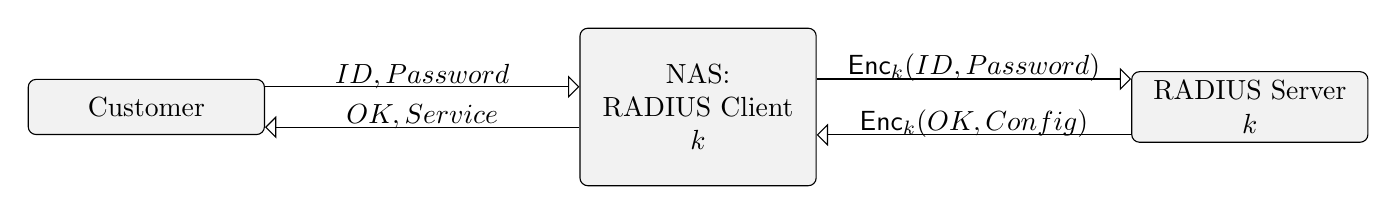
\begin{tikzpicture}
	\tikzstyle{mybox}=[draw=black,align=center,minimum height=7mm, minimum width=30mm]
    % style variants, can be off-commented
	\tikzstyle{mybox}+=[rounded corners=1mm]
    \tikzstyle{mybox}+=[top color=gray!10, bottom color=gray!10]


    \tikzstyle{myarrow}=[->, >=open triangle 90]

	\tikzstyle{mydesc}=[midway, above=-1ex, anchor=south]
	
	\node[mybox] (kunde) {Customer};
    % minimum height can be removed
	\node[mybox, minimum height=20mm] (nas) at ([xshift=55mm] kunde.east) {NAS: \\ RADIUS Client\\ $k$};
	\node[mybox] (server) at ([xshift=55mm] nas.east) {RADIUS Server \\ $k$};
	
	\draw[myarrow] ([yshift=-1mm] kunde.north east) -- ([yshift=-1mm] nas.west |- kunde.north) node[mydesc] {$ID, Password$};
	
	\draw[myarrow,<-] ([yshift=1mm] kunde.south east) -- ([yshift=1mm] nas.west |- kunde.south) node[mydesc] {$OK, Service$};
	
		
	\draw[myarrow] ([yshift=-1mm] nas.east |- server.north) -- ([yshift=-1mm] server.north west) node[mydesc] {$\mathsf{Enc}_k(ID,Password)$};
		
	\draw[myarrow,<-] ([yshift=1mm] nas.east |- server.south) -- ([yshift=1mm] server.south west) node[mydesc] {$\mathsf{Enc}_k(OK, Config)$};
		
\end{tikzpicture}
    
\end{document}
